% Options for packages loaded elsewhere
\PassOptionsToPackage{unicode}{hyperref}
\PassOptionsToPackage{hyphens}{url}
%
\documentclass[
]{article}
\usepackage{lmodern}
\usepackage{amssymb,amsmath}
\usepackage{ifxetex,ifluatex}
\ifnum 0\ifxetex 1\fi\ifluatex 1\fi=0 % if pdftex
  \usepackage[T1]{fontenc}
  \usepackage[utf8]{inputenc}
  \usepackage{textcomp} % provide euro and other symbols
\else % if luatex or xetex
  \usepackage{unicode-math}
  \defaultfontfeatures{Scale=MatchLowercase}
  \defaultfontfeatures[\rmfamily]{Ligatures=TeX,Scale=1}
\fi
% Use upquote if available, for straight quotes in verbatim environments
\IfFileExists{upquote.sty}{\usepackage{upquote}}{}
\IfFileExists{microtype.sty}{% use microtype if available
  \usepackage[]{microtype}
  \UseMicrotypeSet[protrusion]{basicmath} % disable protrusion for tt fonts
}{}
\makeatletter
\@ifundefined{KOMAClassName}{% if non-KOMA class
  \IfFileExists{parskip.sty}{%
    \usepackage{parskip}
  }{% else
    \setlength{\parindent}{0pt}
    \setlength{\parskip}{6pt plus 2pt minus 1pt}}
}{% if KOMA class
  \KOMAoptions{parskip=half}}
\makeatother
\usepackage{xcolor}
\IfFileExists{xurl.sty}{\usepackage{xurl}}{} % add URL line breaks if available
\IfFileExists{bookmark.sty}{\usepackage{bookmark}}{\usepackage{hyperref}}
\hypersetup{
  pdftitle={Statistical Learning and Data Analysis 2021 - 52525},
  pdfauthor={Abigail Gutman and Shahar Shalom},
  hidelinks,
  pdfcreator={LaTeX via pandoc}}
\urlstyle{same} % disable monospaced font for URLs
\usepackage[margin=1in]{geometry}
\usepackage{color}
\usepackage{fancyvrb}
\newcommand{\VerbBar}{|}
\newcommand{\VERB}{\Verb[commandchars=\\\{\}]}
\DefineVerbatimEnvironment{Highlighting}{Verbatim}{commandchars=\\\{\}}
% Add ',fontsize=\small' for more characters per line
\usepackage{framed}
\definecolor{shadecolor}{RGB}{248,248,248}
\newenvironment{Shaded}{\begin{snugshade}}{\end{snugshade}}
\newcommand{\AlertTok}[1]{\textcolor[rgb]{0.94,0.16,0.16}{#1}}
\newcommand{\AnnotationTok}[1]{\textcolor[rgb]{0.56,0.35,0.01}{\textbf{\textit{#1}}}}
\newcommand{\AttributeTok}[1]{\textcolor[rgb]{0.77,0.63,0.00}{#1}}
\newcommand{\BaseNTok}[1]{\textcolor[rgb]{0.00,0.00,0.81}{#1}}
\newcommand{\BuiltInTok}[1]{#1}
\newcommand{\CharTok}[1]{\textcolor[rgb]{0.31,0.60,0.02}{#1}}
\newcommand{\CommentTok}[1]{\textcolor[rgb]{0.56,0.35,0.01}{\textit{#1}}}
\newcommand{\CommentVarTok}[1]{\textcolor[rgb]{0.56,0.35,0.01}{\textbf{\textit{#1}}}}
\newcommand{\ConstantTok}[1]{\textcolor[rgb]{0.00,0.00,0.00}{#1}}
\newcommand{\ControlFlowTok}[1]{\textcolor[rgb]{0.13,0.29,0.53}{\textbf{#1}}}
\newcommand{\DataTypeTok}[1]{\textcolor[rgb]{0.13,0.29,0.53}{#1}}
\newcommand{\DecValTok}[1]{\textcolor[rgb]{0.00,0.00,0.81}{#1}}
\newcommand{\DocumentationTok}[1]{\textcolor[rgb]{0.56,0.35,0.01}{\textbf{\textit{#1}}}}
\newcommand{\ErrorTok}[1]{\textcolor[rgb]{0.64,0.00,0.00}{\textbf{#1}}}
\newcommand{\ExtensionTok}[1]{#1}
\newcommand{\FloatTok}[1]{\textcolor[rgb]{0.00,0.00,0.81}{#1}}
\newcommand{\FunctionTok}[1]{\textcolor[rgb]{0.00,0.00,0.00}{#1}}
\newcommand{\ImportTok}[1]{#1}
\newcommand{\InformationTok}[1]{\textcolor[rgb]{0.56,0.35,0.01}{\textbf{\textit{#1}}}}
\newcommand{\KeywordTok}[1]{\textcolor[rgb]{0.13,0.29,0.53}{\textbf{#1}}}
\newcommand{\NormalTok}[1]{#1}
\newcommand{\OperatorTok}[1]{\textcolor[rgb]{0.81,0.36,0.00}{\textbf{#1}}}
\newcommand{\OtherTok}[1]{\textcolor[rgb]{0.56,0.35,0.01}{#1}}
\newcommand{\PreprocessorTok}[1]{\textcolor[rgb]{0.56,0.35,0.01}{\textit{#1}}}
\newcommand{\RegionMarkerTok}[1]{#1}
\newcommand{\SpecialCharTok}[1]{\textcolor[rgb]{0.00,0.00,0.00}{#1}}
\newcommand{\SpecialStringTok}[1]{\textcolor[rgb]{0.31,0.60,0.02}{#1}}
\newcommand{\StringTok}[1]{\textcolor[rgb]{0.31,0.60,0.02}{#1}}
\newcommand{\VariableTok}[1]{\textcolor[rgb]{0.00,0.00,0.00}{#1}}
\newcommand{\VerbatimStringTok}[1]{\textcolor[rgb]{0.31,0.60,0.02}{#1}}
\newcommand{\WarningTok}[1]{\textcolor[rgb]{0.56,0.35,0.01}{\textbf{\textit{#1}}}}
\usepackage{graphicx,grffile}
\makeatletter
\def\maxwidth{\ifdim\Gin@nat@width>\linewidth\linewidth\else\Gin@nat@width\fi}
\def\maxheight{\ifdim\Gin@nat@height>\textheight\textheight\else\Gin@nat@height\fi}
\makeatother
% Scale images if necessary, so that they will not overflow the page
% margins by default, and it is still possible to overwrite the defaults
% using explicit options in \includegraphics[width, height, ...]{}
\setkeys{Gin}{width=\maxwidth,height=\maxheight,keepaspectratio}
% Set default figure placement to htbp
\makeatletter
\def\fps@figure{htbp}
\makeatother
\setlength{\emergencystretch}{3em} % prevent overfull lines
\providecommand{\tightlist}{%
  \setlength{\itemsep}{0pt}\setlength{\parskip}{0pt}}
\setcounter{secnumdepth}{-\maxdimen} % remove section numbering
\usepackage{booktabs}
\usepackage{longtable}
\usepackage{array}
\usepackage{multirow}
\usepackage{wrapfig}
\usepackage{float}
\usepackage{colortbl}
\usepackage{pdflscape}
\usepackage{tabu}
\usepackage{threeparttable}
\usepackage{threeparttablex}
\usepackage[normalem]{ulem}
\usepackage{makecell}
\usepackage{xcolor}

\title{Statistical Learning and Data Analysis 2021 - 52525}
\usepackage{etoolbox}
\makeatletter
\providecommand{\subtitle}[1]{% add subtitle to \maketitle
  \apptocmd{\@title}{\par {\large #1 \par}}{}{}
}
\makeatother
\subtitle{Lab 1 - Flights data}
\author{Abigail Gutman and Shahar Shalom}
\date{22/3/2021}

\begin{document}
\maketitle

\begin{Shaded}
\begin{Highlighting}[]
\KeywordTok{options}\NormalTok{(}\DataTypeTok{scipen =} \DecValTok{999}\NormalTok{)}
\NormalTok{flights <-}\StringTok{ }\KeywordTok{as.data.frame}\NormalTok{(nycflights13}\OperatorTok{::}\NormalTok{flights)}
\NormalTok{wheather <-}\StringTok{ }\NormalTok{nycflights13}\OperatorTok{::}\NormalTok{weather}
\NormalTok{airports <-}\StringTok{ }\NormalTok{nycflights13}\OperatorTok{::}\NormalTok{airports}
\NormalTok{planes <-}\StringTok{ }\NormalTok{nycflights13}\OperatorTok{::}\NormalTok{planes}
\end{Highlighting}
\end{Shaded}

\hypertarget{graph-critique}{%
\section{\texorpdfstring{\textbf{1. Graph
Critique}}{1. Graph Critique}}\label{graph-critique}}

\hypertarget{question-1}{%
\subsubsection{Question 1:}\label{question-1}}

The first graph shows us the percentage of flights that departed over a
15-minute delay divided into each destination individually. The purpose
of this graph is to make the reader's eye quickly find the percentage of
flights based on a visualization of the United States map.

The second graph shows the weekly flight cycles throughout 2008 where
the blue line indicates the total number of flights that took off that
day and the red line indicates the number of flights in which there was
a delay of over 15 minutes.

\hypertarget{question-2}{%
\subsubsection{Question 2:}\label{question-2}}

In the first graph the information is not presented in an ideal way, it
is difficult for the reader to identify where each line is coming from,
although it is possible to understand which countries it is but it is
not always possible to identify exactly which airport it is.

In the second graph, in our opinion, the amount of lines and points
confuses the reader and makes it difficult for him to identify the
patterns of flight delays throughout the seasons. In addition, the
information overload makes it difficult to identify recurring latency
patterns on certain days for the length of the weekly / monthly cycle.

\hypertarget{question-3}{%
\subsubsection{Question 3:}\label{question-3}}

The first graph raises the obvious question: Are there countries where
the average latency is higher than in other countries? In addition,
which are the airports where the percentage of delays is higher? Another
question is whether the percentages of delay measured vary according to
the seasons?

The second graph raises the questions: Are there patterns of lateness
that recur on certain days of the week or in a particular season, or are
there lateness in some months than in other months? In addition, if the
observation was lower by day / month, it would be possible to compare
percentages and learn from the data by comparing proportions.

\hypertarget{question-4}{%
\subsubsection{Question 4:}\label{question-4}}

The first graph can be improved by changing the graph to a dynamic
graph. This means that when the mouse points to a certain line, we will
be presented with the values of the airport we are pointing to.

In the second graph it was possible to improve the visualization by
changing the red bars to a long line connecting the dots which makes it
possible to identify patterns in the delays of the flights.

\hypertarget{reproducing-these-analyses}{%
\section{\texorpdfstring{\textbf{2. Reproducing these
analyses}}{2. Reproducing these analyses}}\label{reproducing-these-analyses}}

\hypertarget{question-1-1}{%
\subsubsection{Question 1:}\label{question-1-1}}

A graphic summarizing the flight volume and flights delayed, broken by
day and showing weekly cycles.

\begin{Shaded}
\begin{Highlighting}[]
\CommentTok{#EWR/ LGA/ JFK to choose}
\NormalTok{week_cycles <-}\StringTok{ }\KeywordTok{as.data.frame}\NormalTok{(flights) }\OperatorTok\StringTok{ }\KeywordTok{filter}\NormalTok{(origin }\OperatorTok{==}\StringTok{ 'EWR'}\NormalTok{) }\OperatorTok\StringTok{ }\NormalTok{dplyr}\OperatorTok{::}\KeywordTok{select}\NormalTok{(time_hour ,dep_delay ,sched_dep_time)}
\NormalTok{week_cycles}\OperatorTok{$}\NormalTok{time_hour <-}\StringTok{ }\KeywordTok{as.Date}\NormalTok{(week_cycles}\OperatorTok{$}\NormalTok{time_hour,}\StringTok{'ddmmmyyyy'}\NormalTok{)}
\NormalTok{week_cycles<-}\StringTok{ }\NormalTok{week_cycles }\OperatorTok\StringTok{ }\KeywordTok{mutate}\NormalTok{(}\DataTypeTok{delay =} \KeywordTok{if_else}\NormalTok{(dep_delay }\OperatorTok{<=}\StringTok{ }\DecValTok{15}\NormalTok{ ,}\DecValTok{0}\NormalTok{,}\DecValTok{1}\NormalTok{,}\DecValTok{0}\NormalTok{))}


\NormalTok{week_cycles_freq <-}\StringTok{ }\NormalTok{week_cycles }\OperatorTok\StringTok{ }\KeywordTok{group_by}\NormalTok{(time_hour) }\OperatorTok\StringTok{ }\KeywordTok{summarise}\NormalTok{(}\DataTypeTok{frequency =} \KeywordTok{n}\NormalTok{())}
\NormalTok{week_cycles_delay <-}\StringTok{ }\NormalTok{week_cycles }\OperatorTok\StringTok{ }\KeywordTok{group_by}\NormalTok{(time_hour) }\OperatorTok\StringTok{ }\KeywordTok{summarise}\NormalTok{(}\KeywordTok{sum}\NormalTok{(delay))}
\NormalTok{l <-}\StringTok{ }\KeywordTok{length}\NormalTok{(week_cycles_freq}\OperatorTok{$}\NormalTok{frequency)}
\NormalTok{week_cycles_min <-}\StringTok{ }\NormalTok{week_cycles_freq[}\KeywordTok{c}\NormalTok{(}\DecValTok{2}\OperatorTok{:}\NormalTok{(l}\DecValTok{-1}\NormalTok{)),]}
\NormalTok{week_cycles_min <-}\StringTok{ }\NormalTok{week_cycles_min }\OperatorTok\StringTok{ }\KeywordTok{mutate}\NormalTok{(}\DataTypeTok{local_min =}\NormalTok{ (week_cycles_min}\OperatorTok{$}\NormalTok{frequency }\OperatorTok{==}\StringTok{ }\KeywordTok{runmin}\NormalTok{(week_cycles_min}\OperatorTok{$}\NormalTok{frequency,}\KeywordTok{length}\NormalTok{(week_cycles_min}\OperatorTok{$}\NormalTok{frequency)}\OperatorTok{/}\FloatTok{1.3}\NormalTok{)))  }
\NormalTok{week_cycles_min <-}\StringTok{ }\NormalTok{week_cycles_min }\OperatorTok\StringTok{ }\KeywordTok{filter}\NormalTok{(local_min }\OperatorTok{==}\StringTok{ }\NormalTok{T) }\OperatorTok\StringTok{ }\KeywordTok{filter}\NormalTok{(frequency }\OperatorTok{<}\StringTok{ }\DecValTok{250}\NormalTok{)}


\NormalTok{p <-}\StringTok{ }\KeywordTok{ggplot}\NormalTok{(}\DataTypeTok{data =}\NormalTok{ week_cycles_freq,}\KeywordTok{aes}\NormalTok{(}\DataTypeTok{x =}\NormalTok{ time_hour,}
                                   \DataTypeTok{y=}\NormalTok{ week_cycles_freq}\OperatorTok{$}\NormalTok{frequency,}\DataTypeTok{colour =} \StringTok{"blue"}\NormalTok{)) }\OperatorTok{+}
\StringTok{  }\KeywordTok{geom_point}\NormalTok{() }\OperatorTok{+}\StringTok{ }\KeywordTok{geom_line}\NormalTok{(}\KeywordTok{aes}\NormalTok{(}\DataTypeTok{color =} \StringTok{"blue"}\NormalTok{)) }\OperatorTok{+}
\StringTok{  }\KeywordTok{geom_point}\NormalTok{(}\DataTypeTok{data =}\NormalTok{ week_cycles_delay,}\KeywordTok{aes}\NormalTok{(}\DataTypeTok{x=}\NormalTok{time_hour,}\DataTypeTok{y=} \StringTok{`}\DataTypeTok{sum(delay)}\StringTok{`}\NormalTok{, }\DataTypeTok{color =}\StringTok{'red'}\NormalTok{)) }\OperatorTok{+}
\StringTok{  }\KeywordTok{geom_linerange}\NormalTok{(}\DataTypeTok{data =}\NormalTok{ week_cycles_delay,}\KeywordTok{aes}\NormalTok{(}\DataTypeTok{x=}\NormalTok{ time_hour, }\DataTypeTok{ymax =}\StringTok{`}\DataTypeTok{sum(delay)}\StringTok{`}\NormalTok{ ,}\DataTypeTok{ymin=}\DecValTok{0}\NormalTok{),}\DataTypeTok{color =} \StringTok{'red'}\NormalTok{) }\OperatorTok{+}
\StringTok{  }\KeywordTok{geom_point}\NormalTok{(}\DataTypeTok{data =}\NormalTok{ week_cycles_min,}\KeywordTok{aes}\NormalTok{(}\DataTypeTok{x=}\NormalTok{time_hour,}\DataTypeTok{y=}\NormalTok{week_cycles_min}\OperatorTok{$}\NormalTok{frequency, }\DataTypeTok{color =} \StringTok{"lightblue"}\NormalTok{),}\DataTypeTok{size =} \DecValTok{7}\NormalTok{)}\OperatorTok{+}
\StringTok{  }\KeywordTok{scale_color_identity}\NormalTok{(}\DataTypeTok{name =}\StringTok{""}\NormalTok{ ,}\DataTypeTok{breaks =} \KeywordTok{c}\NormalTok{(}\StringTok{"blue"}\NormalTok{,}\StringTok{"red"}\NormalTok{, }\StringTok{"lightblue"}\NormalTok{),}
                       \DataTypeTok{labels =} \KeywordTok{c}\NormalTok{(}\StringTok{"All Flights (scheculed for departure)"}\NormalTok{, }
                                  \StringTok{"Late Flights (departure delayed >15)"}\NormalTok{, }\StringTok{"Fewer flights on holidays"}\NormalTok{),}
                          \DataTypeTok{guide =}  \KeywordTok{guide_legend}\NormalTok{(}\DataTypeTok{override.aes =} \KeywordTok{list}\NormalTok{(}\DataTypeTok{linetype =} \KeywordTok{c}\NormalTok{(}\DecValTok{1}\NormalTok{, }\DecValTok{1}\NormalTok{, }\DecValTok{0}\NormalTok{), }\DataTypeTok{shape =}                                                        \KeywordTok{c}\NormalTok{(}\DecValTok{16}\NormalTok{,}\DecValTok{16}\NormalTok{,}\DecValTok{16}\NormalTok{),}\DataTypeTok{size =} \KeywordTok{c}\NormalTok{(}\DecValTok{1}\NormalTok{,}\DecValTok{1}\NormalTok{,}\DecValTok{7}\NormalTok{)))) }\OperatorTok{+}\StringTok{ }
\StringTok{  }\KeywordTok{theme_light}\NormalTok{()  }\OperatorTok{+}
\StringTok{  }\KeywordTok{xlab}\NormalTok{(}\StringTok{""}\NormalTok{)}\OperatorTok{+}\StringTok{ }\KeywordTok{ylab}\NormalTok{(}\StringTok{"Flights  }\CharTok{\textbackslash{}n}\StringTok{ per day"}\NormalTok{) }\OperatorTok{+}
\StringTok{  }\KeywordTok{xlim}\NormalTok{(}\KeywordTok{as.Date}\NormalTok{(}\KeywordTok{c}\NormalTok{(}\StringTok{"2013-01-01"}\NormalTok{,}\StringTok{"2014-01-01"}\NormalTok{)))}\OperatorTok{+}\StringTok{  }\KeywordTok{ylim}\NormalTok{(}\KeywordTok{c}\NormalTok{(}\DecValTok{0}\NormalTok{, }\DecValTok{400}\NormalTok{)) }\OperatorTok{+}
\StringTok{  }\KeywordTok{theme}\NormalTok{(}\DataTypeTok{axis.title.y =} \KeywordTok{element_text}\NormalTok{(}\DataTypeTok{angle =} \DecValTok{0}\NormalTok{, }\DataTypeTok{vjust =} \FloatTok{1.1}\NormalTok{, }\DataTypeTok{hjust =} \DecValTok{10}\NormalTok{)) }\OperatorTok{+}
\StringTok{  }\KeywordTok{scale_x_date}\NormalTok{(}\DataTypeTok{date_labels =} \StringTok{"%d%b%Y"}\NormalTok{, }\DataTypeTok{date_breaks =} \StringTok{"1 month"}\NormalTok{,}\DataTypeTok{expand =} \KeywordTok{c}\NormalTok{(}\DecValTok{0}\NormalTok{,}\DecValTok{0}\NormalTok{)) }\OperatorTok{+}\StringTok{ }
\StringTok{  }\KeywordTok{theme}\NormalTok{(}\DataTypeTok{legend.position=}\StringTok{"top"}\NormalTok{,}\DataTypeTok{legend.direction =} \StringTok{"vertical"}\NormalTok{) }\OperatorTok{+}
\StringTok{  }\KeywordTok{ggtitle}\NormalTok{(}\DataTypeTok{label =} \StringTok{"Weekly Cycles"}\NormalTok{, }\DataTypeTok{subtitle =} \StringTok{"the airport = EWR   Year = 2013"}\NormalTok{) }\OperatorTok{+}
\StringTok{  }\KeywordTok{theme}\NormalTok{(}\DataTypeTok{plot.title =} \KeywordTok{element_text}\NormalTok{(}\DataTypeTok{hjust =} \FloatTok{0.5}\NormalTok{,}\DataTypeTok{size =} \DecValTok{20}\NormalTok{),}
        \DataTypeTok{plot.subtitle =} \KeywordTok{element_text}\NormalTok{(}\DataTypeTok{hjust =} \FloatTok{0.5}\NormalTok{,}\DataTypeTok{size =} \DecValTok{15}\NormalTok{))}

\NormalTok{tab <-}\StringTok{ }\KeywordTok{as.data.frame}\NormalTok{(}
  \KeywordTok{c}\NormalTok{(}\StringTok{"<b>}\CharTok{\textbackslash{}n}\StringTok{ WEEKLY CYCLES  }\CharTok{\textbackslash{}n}\StringTok{ FEW FLIGHTS: SUNDAYS AND SATURDAYS }\CharTok{\textbackslash{}n}\StringTok{ MOST FLIGHTS: MONDAYS, THURSDAYS }\CharTok{\textbackslash{}n}\StringTok{ AND FRIDAYS"}\NormalTok{))}
\NormalTok{g <-}\StringTok{ }\KeywordTok{textGrob}\NormalTok{(}\StringTok{"}\CharTok{\textbackslash{}n\textbackslash{}n}\StringTok{ WEEKLY CYCLES  }\CharTok{\textbackslash{}n}\StringTok{ FEW FLIGHTS: }\CharTok{\textbackslash{}n}\StringTok{ SUNDAYS AND SATURDAYS }\CharTok{\textbackslash{}n}
\StringTok{              MOST FLIGHTS: }\CharTok{\textbackslash{}n}\StringTok{ MONDAYS, THURSDAYS }\CharTok{\textbackslash{}n}\StringTok{ AND FRIDAYS"}\NormalTok{, }\DataTypeTok{gp=}\KeywordTok{gpar}\NormalTok{(}\DataTypeTok{fontsize=}\DecValTok{13}\NormalTok{,}\DataTypeTok{font=}\DecValTok{1}\NormalTok{))}
\KeywordTok{grid.arrange}\NormalTok{(g, p, }\DataTypeTok{layout_matrix =} \KeywordTok{matrix}\NormalTok{(}\KeywordTok{c}\NormalTok{(}\DecValTok{1}\NormalTok{,}\DecValTok{2}\NormalTok{,}\DecValTok{2}\NormalTok{, }\DecValTok{2}\NormalTok{, }\DecValTok{2}\NormalTok{), }\DataTypeTok{ncol =} \DecValTok{5}\NormalTok{),}
             \DataTypeTok{top =} \KeywordTok{textGrob}\NormalTok{(}\StringTok{"      TEMPORAL EFFECTS"}\NormalTok{, }\DataTypeTok{gp=}\KeywordTok{gpar}\NormalTok{(}\DataTypeTok{fontsize=}\DecValTok{30}\NormalTok{,}\DataTypeTok{font=}\DecValTok{1}\NormalTok{)))}
\end{Highlighting}
\end{Shaded}

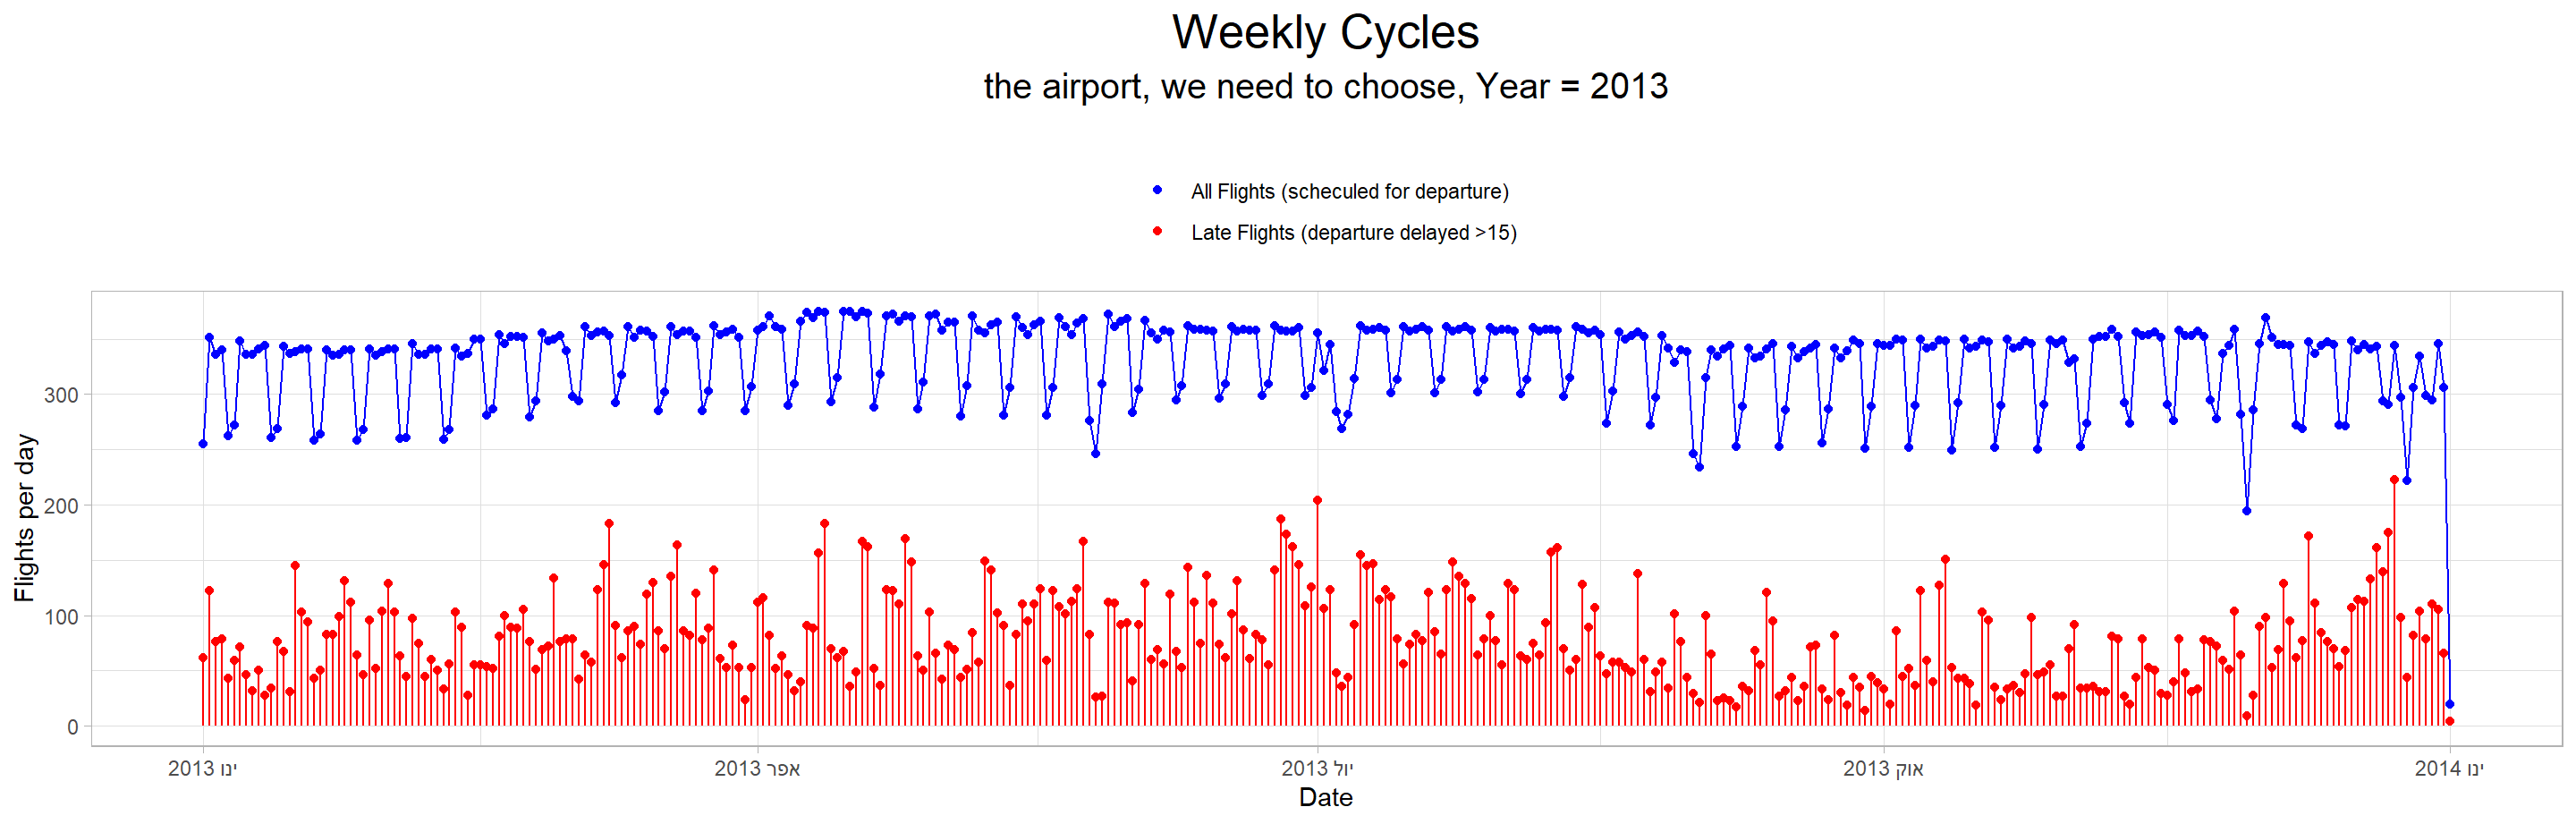
\includegraphics{Statistical_Learning_Lab_1_files/figure-latex/fig3-1.pdf}

\hypertarget{question-2-1}{%
\subsubsection{Question 2:}\label{question-2-1}}

The other graph, flight percent

\begin{Shaded}
\begin{Highlighting}[]
\NormalTok{dep_delay <-}\StringTok{ }\KeywordTok{as.data.frame}\NormalTok{(flights) }\OperatorTok\StringTok{ }\KeywordTok{filter}\NormalTok{(origin }\OperatorTok{==}\StringTok{ 'JFK'}\NormalTok{) }\OperatorTok\StringTok{ }\KeywordTok{group_by}\NormalTok{(dest) }\OperatorTok
\StringTok{  }\KeywordTok{count}\NormalTok{()}
\KeywordTok{colnames}\NormalTok{(dep_delay) <-}\KeywordTok{c}\NormalTok{(}\StringTok{"faa"}\NormalTok{, }\StringTok{"amount"}\NormalTok{)}

\NormalTok{dep_delay2 <-}\StringTok{ }\KeywordTok{as.data.frame}\NormalTok{(flights) }\OperatorTok\StringTok{ }\KeywordTok{filter}\NormalTok{(origin }\OperatorTok{==}\StringTok{ 'JFK'}\NormalTok{) }\OperatorTok\StringTok{ }\KeywordTok{group_by}\NormalTok{(dest) }\OperatorTok\StringTok{ }\KeywordTok{filter}\NormalTok{(dep_delay }\OperatorTok{>}\DecValTok{15}\NormalTok{) }\OperatorTok\StringTok{   }\KeywordTok{count}\NormalTok{()}
\KeywordTok{colnames}\NormalTok{(dep_delay2) <-}\StringTok{ }\KeywordTok{c}\NormalTok{(}\StringTok{"faa"}\NormalTok{,}\StringTok{"delay"}\NormalTok{)}

\NormalTok{dep_delay <-}\StringTok{ }\NormalTok{dep_delay }\OperatorTok\StringTok{ }\KeywordTok{left_join}\NormalTok{(dep_delay2) }\OperatorTok\StringTok{ }\KeywordTok{mutate}\NormalTok{(}\DataTypeTok{per =}\NormalTok{ delay}\OperatorTok{/}\StringTok{ }\NormalTok{amount)}

\NormalTok{dep_delay_loc <-}\StringTok{ }\NormalTok{dep_delay }\OperatorTok\StringTok{ }\KeywordTok{left_join}\NormalTok{(airports, }\DataTypeTok{by =} \StringTok{"faa"}\NormalTok{) }\OperatorTok\StringTok{ }\KeywordTok{drop_na}\NormalTok{()}
\CommentTok{# removed : STT,SJU, BQN need to be explain why they can be found.}
\NormalTok{dep_delay_loc <-}\StringTok{ }\NormalTok{dep_delay_loc }\OperatorTok\StringTok{ }\KeywordTok{mutate}\NormalTok{(}\DataTypeTok{per_ch =} \OtherTok{NA}\NormalTok{)}
\NormalTok{dep_delay_loc}\OperatorTok{$}\NormalTok{per_ch[dep_delay_loc}\OperatorTok{$}\NormalTok{per }\OperatorTok{<=}\StringTok{ }\FloatTok{0.10}\NormalTok{ ] <-}\StringTok{ "<= 10%"}
\NormalTok{dep_delay_loc}\OperatorTok{$}\NormalTok{per_ch[dep_delay_loc}\OperatorTok{$}\NormalTok{per }\OperatorTok{<=}\StringTok{ }\FloatTok{0.15} \OperatorTok{&}\StringTok{ }\NormalTok{dep_delay_loc}\OperatorTok{$}\NormalTok{per }\OperatorTok{>}\StringTok{ }\FloatTok{0.10}\NormalTok{ ] <-}\StringTok{ "10% - 15%"}
\NormalTok{dep_delay_loc}\OperatorTok{$}\NormalTok{per_ch[dep_delay_loc}\OperatorTok{$}\NormalTok{per }\OperatorTok{<=}\StringTok{ }\FloatTok{0.20} \OperatorTok{&}\StringTok{ }\NormalTok{dep_delay_loc}\OperatorTok{$}\NormalTok{per }\OperatorTok{>}\StringTok{ }\FloatTok{0.15}\NormalTok{ ] <-}\StringTok{ "15% - 20%"}
\NormalTok{dep_delay_loc}\OperatorTok{$}\NormalTok{per_ch[dep_delay_loc}\OperatorTok{$}\NormalTok{per }\OperatorTok{<=}\StringTok{ }\FloatTok{0.25} \OperatorTok{&}\StringTok{ }\NormalTok{dep_delay_loc}\OperatorTok{$}\NormalTok{per }\OperatorTok{>}\StringTok{ }\FloatTok{0.20}\NormalTok{ ] <-}\StringTok{ "20% - 25%"}
\NormalTok{dep_delay_loc}\OperatorTok{$}\NormalTok{per_ch[dep_delay_loc}\OperatorTok{$}\NormalTok{per }\OperatorTok{>=}\StringTok{ }\FloatTok{0.25}\NormalTok{] <-}\StringTok{ "25% <="}
\NormalTok{dep_delay_loc}\OperatorTok{$}\NormalTok{per_ch <-}\StringTok{ }\KeywordTok{factor}\NormalTok{(dep_delay_loc}\OperatorTok{$}\NormalTok{per_ch, }\DataTypeTok{levels =} \KeywordTok{c}\NormalTok{(}\StringTok{"<= 10%"}\NormalTok{,}\StringTok{"10% - 15%"}\NormalTok{,}
                                                         \StringTok{"15% - 20%"}\NormalTok{,}\StringTok{"20% - 25%"}\NormalTok{,}\StringTok{"25% <="}\NormalTok{))}
\end{Highlighting}
\end{Shaded}

\begin{Shaded}
\begin{Highlighting}[]
\NormalTok{dep_delay_loc <-}\StringTok{ }\NormalTok{dep_delay_loc }\OperatorTok\StringTok{ }\KeywordTok{mutate}\NormalTok{(}\DataTypeTok{nyc_EWR_lon =} \FloatTok{-74.16867}\NormalTok{) }\OperatorTok
\StringTok{  }\KeywordTok{mutate}\NormalTok{(}\DataTypeTok{nyc_EWR_lat =} \FloatTok{40.6925}\NormalTok{ )}


\NormalTok{dep_delay_loc <-}\StringTok{ }\KeywordTok{as.data.frame}\NormalTok{(dep_delay_loc)}

\NormalTok{dep_delay_trans <-}\StringTok{ }\NormalTok{dep_delay_loc }\OperatorTok
\StringTok{  }\KeywordTok{select}\NormalTok{(lon,lat) }\OperatorTok\StringTok{ }\KeywordTok{usmap_transform}\NormalTok{()}
\NormalTok{dep_delay_loc}\OperatorTok{$}\NormalTok{lon <-}\StringTok{ }\NormalTok{dep_delay_trans}\OperatorTok{$}\NormalTok{lon}\FloatTok{.1}
\NormalTok{dep_delay_loc}\OperatorTok{$}\NormalTok{lat <-}\StringTok{ }\NormalTok{dep_delay_trans}\OperatorTok{$}\NormalTok{lat}\FloatTok{.1}

\NormalTok{dep_delay_trans <-}\StringTok{ }\NormalTok{dep_delay_loc }\OperatorTok\StringTok{ }\KeywordTok{select}\NormalTok{(nyc_EWR_lon,nyc_EWR_lat) }\OperatorTok\StringTok{ }\KeywordTok{usmap_transform}\NormalTok{()}
\NormalTok{dep_delay_loc}\OperatorTok{$}\NormalTok{lnyc_EWR_lon <-}\StringTok{ }\NormalTok{dep_delay_trans}\OperatorTok{$}\NormalTok{nyc_EWR_lon}\FloatTok{.1}
\NormalTok{dep_delay_loc}\OperatorTok{$}\NormalTok{lnyc_EWR_lat <-}\StringTok{ }\NormalTok{dep_delay_trans}\OperatorTok{$}\NormalTok{nyc_EWR_lat}\FloatTok{.1}
\KeywordTok{row.names}\NormalTok{(dep_delay_loc) <-}\StringTok{ }\NormalTok{dep_delay_loc}\OperatorTok{$}\NormalTok{name}

\NormalTok{plot_del <-}\StringTok{ }\KeywordTok{plot_usmap}\NormalTok{(}\DataTypeTok{regions =} \StringTok{"states"}\NormalTok{,}\DataTypeTok{labels =} \OtherTok{TRUE}\NormalTok{,}\DataTypeTok{exclude =}  \KeywordTok{c}\NormalTok{(}\StringTok{"AK"}\NormalTok{,}\StringTok{"HI"}\NormalTok{), }\DataTypeTok{size =} \FloatTok{0.5}\NormalTok{,}
           \DataTypeTok{label_color =} \StringTok{"grey"}\NormalTok{,}
           \DataTypeTok{color =} \StringTok{"grey"}\NormalTok{) }\OperatorTok{+}\StringTok{ }
\StringTok{    }\KeywordTok{theme}\NormalTok{(}\DataTypeTok{panel.background=}\KeywordTok{element_blank}\NormalTok{()) }\OperatorTok{+}
\StringTok{  }\KeywordTok{geom_segment}\NormalTok{(}\DataTypeTok{data =}\NormalTok{ dep_delay_loc,}
               \KeywordTok{aes}\NormalTok{(}\DataTypeTok{xend =}\NormalTok{ lon,}\DataTypeTok{yend =}\NormalTok{ lat, }\DataTypeTok{x =}\NormalTok{ lnyc_EWR_lon,}
                                         \DataTypeTok{y =}\NormalTok{ lnyc_EWR_lat ,}\DataTypeTok{colour =}\NormalTok{ per_ch),}\DataTypeTok{size =} \FloatTok{0.5}\NormalTok{) }\OperatorTok{+}\StringTok{ }
\StringTok{  }\KeywordTok{geom_point}\NormalTok{(}\DataTypeTok{data =}\NormalTok{ dep_delay_loc,}
             \KeywordTok{aes}\NormalTok{(}\DataTypeTok{x =}\NormalTok{ lon , }\DataTypeTok{y =}\NormalTok{ lat, }\DataTypeTok{colour =}\NormalTok{  per_ch,}
                 \DataTypeTok{text =} \KeywordTok{row.names}\NormalTok{(dep_delay_loc)),}
             \DataTypeTok{size =} \FloatTok{0.5}\NormalTok{, }\DataTypeTok{show.legend =}\NormalTok{ F) }\OperatorTok{+}
\StringTok{  }\KeywordTok{scale_color_manual}\NormalTok{(}\DataTypeTok{name =} \StringTok{""}\NormalTok{,}
                     \DataTypeTok{values =} \KeywordTok{c}\NormalTok{(}\StringTok{"green"}\NormalTok{,}\StringTok{"purple"}\NormalTok{,}\StringTok{"blue"}\NormalTok{,}\StringTok{"orange"}\NormalTok{,}\StringTok{"red"}\NormalTok{),}
                     \DataTypeTok{guide =}  \KeywordTok{guide_legend}\NormalTok{(}\DataTypeTok{override.aes =} \KeywordTok{list}\NormalTok{(}\DataTypeTok{linetype =} \KeywordTok{c}\NormalTok{(}\DecValTok{1}\NormalTok{, }\DecValTok{1}\NormalTok{, }\DecValTok{1}\NormalTok{,}\DecValTok{1}\NormalTok{,}\DecValTok{1}\NormalTok{), }
                                          \DataTypeTok{size =} \KeywordTok{c}\NormalTok{(}\DecValTok{2}\NormalTok{,}\DecValTok{2}\NormalTok{,}\DecValTok{2}\NormalTok{,}\DecValTok{2}\NormalTok{,}\DecValTok{2}\NormalTok{))))}\OperatorTok{+}
\StringTok{    }\KeywordTok{labs}\NormalTok{(}\DataTypeTok{title =} \StringTok{'<b>% of Flight Departures Delayed > 15 Min</b><br> Airport = JFK Year = 2013<br><br><br><br><br><br><br><br><br><br><br><br><br><br><br><br><br><br><br> Click line endpoint to see that airports departures'}\NormalTok{) }\OperatorTok{+}
\StringTok{      }\KeywordTok{theme}\NormalTok{(}\DataTypeTok{plot.title =} \KeywordTok{element_text}\NormalTok{(}\DataTypeTok{hjust =} \FloatTok{0.5}\NormalTok{,}\DataTypeTok{size =} \DecValTok{12}\NormalTok{))}

\NormalTok{plot_del}\OperatorTok{$}\NormalTok{x}\OperatorTok{$}\NormalTok{data[[}\DecValTok{1}\NormalTok{]]}\OperatorTok{$}\NormalTok{hoverinfo <-}\StringTok{ "none"}
\NormalTok{plot_del}\OperatorTok{$}\NormalTok{y}\OperatorTok{$}\NormalTok{data[[}\DecValTok{1}\NormalTok{]]}\OperatorTok{$}\NormalTok{hoverinfo <-}\StringTok{ "none"}

\KeywordTok{ggplotly}\NormalTok{(plot_del, }\DataTypeTok{tooltip =} \StringTok{"text"}\NormalTok{) }\OperatorTok\StringTok{ }\KeywordTok{layout}\NormalTok{(}\DataTypeTok{legend =} \KeywordTok{list}\NormalTok{(}\DataTypeTok{x =} \DecValTok{0}\NormalTok{, }\DataTypeTok{y =} \DecValTok{0}\NormalTok{))}
\end{Highlighting}
\end{Shaded}

\includegraphics{Statistical_Learning_Lab_1_files/figure-latex/unnamed-chunk-3-1.pdf}

Note that the \texttt{echo\ =\ FALSE} parameter was added to the code
chunk to prevent printing of the R code that generated the plot.

\hypertarget{freestyle-analysis}{%
\section{\texorpdfstring{\textbf{3. Freestyle
analysis:}}{3. Freestyle analysis:}}\label{freestyle-analysis}}

The first graph shows the relationship between visibility and flight
delays.

\begin{Shaded}
\begin{Highlighting}[]
\NormalTok{flights_delayed <-}\StringTok{ }\KeywordTok{filter}\NormalTok{(flights, dep_delay }\OperatorTok{>}\DecValTok{15}\NormalTok{ ) }\CommentTok{#We want to see only the delayed flights }
\NormalTok{flights_delayed1 <-}\StringTok{ }\NormalTok{flights_delayed }\OperatorTok\StringTok{  }\KeywordTok{group_by}\NormalTok{(time_hour) }\OperatorTok\StringTok{ }\KeywordTok{summarise}\NormalTok{(}\DataTypeTok{Avg_dep_delay =} \KeywordTok{mean}\NormalTok{(dep_delay))}

\NormalTok{Wheather_cond <-}\StringTok{ }\KeywordTok{left_join}\NormalTok{(flights_delayed1, wheather) }\CommentTok{#combine the two relevant data frames }

\CommentTok{#aggregate the data so we can see the conection between visib to avg sep delay.}
\NormalTok{visib_df <-}\StringTok{ }\NormalTok{Wheather_cond }\OperatorTok\StringTok{ }\KeywordTok{group_by}\NormalTok{(visib) }\OperatorTok\StringTok{ }\KeywordTok{summarise}\NormalTok{(}\DataTypeTok{Avg_dep_delay =} \KeywordTok{mean}\NormalTok{(Avg_dep_delay, }\DataTypeTok{na.rm =}\NormalTok{ T), }\DataTypeTok{n =} \KeywordTok{n}\NormalTok{())}
\NormalTok{visib_df <-}\StringTok{ }\NormalTok{visib_df }\OperatorTok\StringTok{ }\KeywordTok{filter}\NormalTok{(n }\OperatorTok{>}\StringTok{ }\DecValTok{30}\NormalTok{)}

\KeywordTok{ggplot}\NormalTok{(}\DataTypeTok{data =}\NormalTok{ visib_df, }\DataTypeTok{mapping =} \KeywordTok{aes}\NormalTok{(}\DataTypeTok{x =}\NormalTok{ visib, }\DataTypeTok{y =}\NormalTok{ Avg_dep_delay)) }\OperatorTok{+}\StringTok{ }\KeywordTok{geom_point}\NormalTok{(}\DataTypeTok{color =} \StringTok{"violetred4"}\NormalTok{) }\OperatorTok{+}\StringTok{ }
\StringTok{  }\KeywordTok{geom_smooth}\NormalTok{(}\DataTypeTok{method =} \StringTok{"lm"}\NormalTok{, }\DataTypeTok{fill =} \StringTok{"violet"}\NormalTok{, }\DataTypeTok{color =} \StringTok{"violetred4"}\NormalTok{) }\OperatorTok{+}
\StringTok{  }\KeywordTok{labs}\NormalTok{(}\DataTypeTok{x =} \StringTok{"visibility"}\NormalTok{, }\DataTypeTok{y=}\StringTok{"Average Departure Delay Time (minutes)"}\NormalTok{, }\DataTypeTok{title =} \StringTok{"Average Departure Delay vs. Quality of visibility"}\NormalTok{)}
\end{Highlighting}
\end{Shaded}

\includegraphics{Statistical_Learning_Lab_1_files/figure-latex/unnamed-chunk-4-1.pdf}

When we tried to think what was the main reason for the delay of flights
the first thing that came to our mind was the weather conditions. When
we studied the weather database we noticed a variable called ``visib''
and decided to try to understand the relationship between visibility and
flight delays. The graph shown above shows a direct relationship between
the quality of visibility and the average flight delay in minutes. The
better the visibility, the smaller the average delays.

\begin{Shaded}
\begin{Highlighting}[]
\CommentTok{#As before we summarise the average delay, only this time we compare it to the wind speed.   }
\NormalTok{by_wind_speed <-}\StringTok{ }\NormalTok{Wheather_cond }\OperatorTok\StringTok{ }\KeywordTok{group_by}\NormalTok{(wind_speed) }\OperatorTok\StringTok{ }\KeywordTok{summarise}\NormalTok{(}\DataTypeTok{Avg_dep_delay =} \KeywordTok{mean}\NormalTok{(Avg_dep_delay, }\DataTypeTok{na.rm =}\NormalTok{ T), }\DataTypeTok{n =} \KeywordTok{n}\NormalTok{())}
\CommentTok{#we filtered average values of less then 30 samples. }
\NormalTok{by_wind_speed <-}\StringTok{  }\KeywordTok{filter}\NormalTok{(by_wind_speed, n}\OperatorTok{>}\DecValTok{30}\NormalTok{)}

\KeywordTok{ggplot}\NormalTok{(}\DataTypeTok{data =}\NormalTok{ by_wind_speed, }\DataTypeTok{mapping =} \KeywordTok{aes}\NormalTok{(}\DataTypeTok{x =}\NormalTok{ wind_speed, }\DataTypeTok{y =}\NormalTok{ Avg_dep_delay)) }\OperatorTok{+}
\StringTok{  }\KeywordTok{geom_point}\NormalTok{(}\DataTypeTok{color =} \StringTok{"dodgerblue4"}\NormalTok{) }\OperatorTok{+}\StringTok{ }
\StringTok{  }\KeywordTok{geom_smooth}\NormalTok{(}\DataTypeTok{method =} \StringTok{"lm"}\NormalTok{, }\DataTypeTok{fill =} \StringTok{"deepskyblue"}\NormalTok{, }\DataTypeTok{color =} \StringTok{"dodgerblue4"}\NormalTok{) }\OperatorTok{+}
\StringTok{  }\KeywordTok{labs}\NormalTok{(}\DataTypeTok{x =} \StringTok{"Wind_speed (mph)"}\NormalTok{, }\DataTypeTok{y=}\StringTok{"Average Departure Delay Time (minutes)"}\NormalTok{, }
       \DataTypeTok{title =} \StringTok{"Average Departure Delay vs. Wind speed"}\NormalTok{)}
\end{Highlighting}
\end{Shaded}

\includegraphics{Statistical_Learning_Lab_1_files/figure-latex/unnamed-chunk-5-1.pdf}

The second graph shows us another interesting relationship between the
weather and the average of flight delays. In the graph above it we can
see positive linear conection between the wind speed and the average
flight delay in minutes. As the wind speed increases the delay time of
the flight also increases.

\hypertarget{graphical-lineup}{%
\section{\texorpdfstring{\textbf{4. Graphical
Lineup:}}{4. Graphical Lineup:}}\label{graphical-lineup}}

\hypertarget{question-1-2}{%
\subsubsection{Question 1:}\label{question-1-2}}

\begin{Shaded}
\begin{Highlighting}[]
\CommentTok{#Creat a plot that shows the distribution of the delayed flights in each day of every month }
\KeywordTok{ggplot}\NormalTok{(}\DataTypeTok{data =}\NormalTok{ flights_delayed, }\KeywordTok{aes}\NormalTok{(}\DataTypeTok{x =}\NormalTok{ day)) }\OperatorTok{+}
\StringTok{  }\KeywordTok{geom_bar}\NormalTok{(}\KeywordTok{aes}\NormalTok{(}\DataTypeTok{fill =}\NormalTok{ month))}\OperatorTok{+}\StringTok{ }\KeywordTok{facet_wrap}\NormalTok{(}\OperatorTok{~}\NormalTok{month) }\OperatorTok{+}\StringTok{ }
\StringTok{  }\KeywordTok{labs}\NormalTok{(}\DataTypeTok{title  =} \StringTok{"Distribution of delayed flight in each month"}\NormalTok{,}
       \DataTypeTok{subtitle =} \StringTok{"(Delayed flights are set to be flights that left the airport with over 15 minutes delay)"}\NormalTok{, }\DataTypeTok{y =} \StringTok{"Number of delayed flight"}\NormalTok{, }\DataTypeTok{x =} \StringTok{"Day"}\NormalTok{) }\OperatorTok{+}\StringTok{ }\KeywordTok{scale_fill_viridis_c}\NormalTok{(}\DataTypeTok{guide =}\NormalTok{ F)}
\end{Highlighting}
\end{Shaded}

\includegraphics{Statistical_Learning_Lab_1_files/figure-latex/unnamed-chunk-6-1.pdf}

In this question we were asked to produce a graph which answers the
question: Is the proportion of delayed flights per month is independent
across months. To this end, we have created a graph that shows for each
month the distribution of flights that have been delayed for more than
15 minutes.

After thoroughly researching the graph findings we came to the
conclusion that there is no relationship between the distribution of the
delayed flights.

As a result of this conclusion it can be said that for these graphs we
will not reject the null hypothesis.

\hypertarget{question-2-2}{%
\subsubsection{Question 2:}\label{question-2-2}}

Before you read the code, stop! Try to think which of the graphs you see
below shows the true distribution of the number of flights that were
delayed each month?

\begin{Shaded}
\begin{Highlighting}[]
\CommentTok{#First' we created a df that containes only the data that we need }
\NormalTok{by_month <-}\StringTok{ }\NormalTok{flights_delayed }\OperatorTok\StringTok{ }\KeywordTok{group_by}\NormalTok{(month) }\OperatorTok\StringTok{ }\KeywordTok{summarise}\NormalTok{(}\DataTypeTok{val =} \KeywordTok{n}\NormalTok{())}
\NormalTok{by_month <-}\StringTok{ }\KeywordTok{data.frame}\NormalTok{(by_month, }\DataTypeTok{semp =} \KeywordTok{c}\NormalTok{(}\KeywordTok{rep}\NormalTok{(}\DecValTok{1}\NormalTok{,}\DecValTok{12}\NormalTok{))) }\CommentTok{#named the real data as sample 1.}

\NormalTok{sampled_df <-}\StringTok{ }\NormalTok{by_month}
\KeywordTok{row.names}\NormalTok{(sampled_df) <-}\StringTok{ }\NormalTok{by_month}\OperatorTok{$}\NormalTok{month}

\CommentTok{#loop that sample new vecrots and tag the sample with number}
\CommentTok{#also each sample will merged to the data that containes the real values. }
\ControlFlowTok{for}\NormalTok{ (i }\ControlFlowTok{in}\NormalTok{ (}\DecValTok{2}\OperatorTok{:}\DecValTok{9}\NormalTok{))\{}
\NormalTok{  x <-}\StringTok{ }\KeywordTok{data.frame}\NormalTok{(}\DataTypeTok{month =} \KeywordTok{c}\NormalTok{(}\DecValTok{1}\OperatorTok{:}\DecValTok{12}\NormalTok{), }\DataTypeTok{semp =} \KeywordTok{c}\NormalTok{(}\KeywordTok{rep}\NormalTok{(i,}\DecValTok{12}\NormalTok{)),}\DataTypeTok{val =} \KeywordTok{sample}\NormalTok{(by_month}\OperatorTok{$}\NormalTok{val))}
\NormalTok{  sampled_df <-}\StringTok{ }\KeywordTok{full_join}\NormalTok{(sampled_df, x)}
\NormalTok{\}}

\CommentTok{#plot all of the samples in the Line-up method}
\CommentTok{# we added colors that will help us identify the pattern of the values. }
\KeywordTok{ggplot}\NormalTok{(}\DataTypeTok{data =}\NormalTok{ sampled_df, }\DataTypeTok{mapping =} \KeywordTok{aes}\NormalTok{(}\DataTypeTok{x  =}\NormalTok{ month, }\DataTypeTok{y =}\NormalTok{ val, }\DataTypeTok{fill =}\NormalTok{ val)) }\OperatorTok{+}\StringTok{ }\KeywordTok{facet_wrap}\NormalTok{(}\OperatorTok{~}\NormalTok{semp) }\OperatorTok{+}
\StringTok{  }\KeywordTok{scale_x_continuous}\NormalTok{(}\DataTypeTok{breaks =} \KeywordTok{c}\NormalTok{(}\DecValTok{1}\OperatorTok{:}\DecValTok{12}\NormalTok{)) }\OperatorTok{+}
\StringTok{  }\KeywordTok{geom_bar}\NormalTok{(}\DataTypeTok{stat=}\StringTok{"identity"}\NormalTok{) }\OperatorTok{+}\StringTok{ }
\StringTok{  }\KeywordTok{labs}\NormalTok{(}\DataTypeTok{title  =} \StringTok{"Simulated data-sets of delayed flight using line-up"}\NormalTok{,}
       \DataTypeTok{subtitle =} \StringTok{"(Delayed flights are set to be flights that left the airport with over 15 minutes delay)"}\NormalTok{,}
       \DataTypeTok{y =} \StringTok{"Number of delayed flight"}\NormalTok{, }\DataTypeTok{x =} \StringTok{"Month"}\NormalTok{)}\OperatorTok{+}
\StringTok{   }\KeywordTok{theme}\NormalTok{(}\DataTypeTok{axis.text.x =} \KeywordTok{element_text}\NormalTok{(}\DataTypeTok{size =} \DecValTok{8}\NormalTok{)) }\OperatorTok{+}
\StringTok{  }\KeywordTok{scale_fill_distiller}\NormalTok{(}\DataTypeTok{palette =} \StringTok{'RdPu'}\NormalTok{, }\DataTypeTok{direction =}\DecValTok{1}\NormalTok{)}
\end{Highlighting}
\end{Shaded}

\includegraphics{Statistical_Learning_Lab_1_files/figure-latex/unnamed-chunk-7-1.pdf}

In this question we were again asked to try to reject the null
hypothesis but this time by creating graphs which are based on
simulations of the data.

To do this we first checked the number of flights delayed each month.
After that we created a vector that represent this values. The next step
was to create simulation based on this values. we created a graph for
every simulation and tries to see if there is any connection between all
of this semples.

So what are you thinking ? Which of the graphs above is the one that
shows the real data distribution? The real data is displayed in graph
number \ldots.. 1!

\hypertarget{question-3-1}{%
\subsubsection{Question 3:}\label{question-3-1}}

While we created the graph above we choose to mach colors for each bar
that represent the numbers of delayed flights, small number will be
represented with lighter colors and larger numbers with darker colors.
As we can see in sapmle 1 that represent the real values there is a
certain trend between the months, the transition between the colors of
the bars is an easy transition in most cases. There is an upward trend
and there is also a downward trend.

When we look at the other graphs that represent the simulations we fail
to notice a similar trend in any of the graphs. As a result we can say
that there is a connection between the months so again we come to the
conclusion that the null hypothesis cannot be rejected.

Finally, we learned that one can learn about relationships between
variables not necessarily with the help of formulas and numbers. Visual
objects can also provide us with a great deal of statistical
information.

\end{document}
